\documentclass[12pt,mathserif,professionalfont]{beamer}

\mode<presentation>
{%
	\usetheme[alternativetitlepage=bild]{Rub}
	\titlegraphic{data/flickr/img-bg.jpg}

	\setbeamercovered{transparent}
}
\usepackage[utf8]{inputenc}
\usepackage[T1]{fontenc}

\usepackage{rubfonts2009}
\usepackage[scaled=.90]{helvet}
\usepackage{courier}
\usepackage{eulervm}
%\usefonttheme[onlymath]{serif}

\usepackage[english]{babel}
\usepackage[babel,english=british]{csquotes}

\usepackage{amsmath}
\usepackage{mathtools}

\usepackage{etoolbox,siunitx}
\sisetup{binary-units}

\usepackage{booktabs}
\usepackage{diagbox}

\usepackage[%
	backend=biber,
	bibencoding=ascii,
	style=numeric,
	sortcites,
	maxbibnames=10,
	maxcitenames=2,
	backref=true,
	firstinits=true,
]{biblatex}
\DefineBibliographyStrings{english}{%
	andothers = {\em et\addabbrvspace{}al\adddot}
}
\DeclareFieldFormat{eprint:iacr}{%
\mkbibacro{iacr}\addcolon\space{}
    \href{https://eprint.iacr.org/#1}{\nolinkurl{#1}}
}
\DeclareFieldFormat{eprint:iacrconf}{%
\mkbibacro{iacr}\addcolon\space{}
    \href{https://www.iacr.org/archive/#1}{\nolinkurl{#1}}
}
\renewcommand\bibfont{\scriptsize}
\bibliography{bibliography}

\newcommand{\blfootnote}[1]{%
	\begingroup
	\renewcommand\thefootnote{}\footnote{#1}%
	\addtocounter{footnote}{-1}%
	\endgroup
}

\DeclarePairedDelimiter\ceil{\lceil}{\rceil}
\DeclarePairedDelimiter\floor{\lfloor}{\rfloor}
\DeclarePairedDelimiter\angleb{\langle}{\rangle}
\DeclarePairedDelimiter\parens{(}{)}
\DeclarePairedDelimiter\bracket{[}{]}
\DeclarePairedDelimiter\curly{\{}{\}}

\DeclareMathOperator*{\argmax}{arg\,max}

\makeatletter
\def\maxwidth#1{\ifdim\Gin@nat@width>#1 #1\else\Gin@nat@width\fi}
\def\maxheight#1{\ifdim\Gin@nat@height>#1 #1\else\Gin@nat@height\fi}
\makeatother

\newcommand{\xor}{\oplus}

\def\present/{\textsc{Present}}
\def\spresent/{\textsc{Small\-Pres\-ent}}
\def\ssaes/{\textsc{Small\-Scale\-AES}}
\def\subbox/{S-box}
\def\subboxes/{S-boxes}

% correct abbreviations http://stackoverflow.com/a/3285603
\usepackage{expl3}
\ExplSyntaxOn{}
\newcommand\latinabbrev[1]{
  \peek_meaning:NTF . {% Same as \@ifnextchar
    #1\@}%
  { \peek_catcode:NTF a {% Check whether next char has same catcode as \'a, i.e., is a letter
      #1.\@ }%
    {#1.\@}}}
\ExplSyntaxOff{}

\def\cf/{\latinabbrev{cf},}
\def\eg/{\latinabbrev{e.\,g},}
\def\etal/{\latinabbrev{\textit{et~al}}}
\def\etc/{\latinabbrev{etc}}
\def\ie/{\latinabbrev{i.\,e},}
\def\resp/{\latinabbrev{resp}}
\def\st/{\latinabbrev{s.\,t}}

\title[On the Influence of the Key Scheduling on Linear Approximations]{On the Influence of the Key Scheduling on\\Linear Approximations}
\subtitle{}
\author[Friedrich~Wiemer]{Friedrich~Wiemer}
\institute{%
	CITS Oberseminar
	%Ruhr University Bochum
}

\date{6. April 2016}

\AtBeginSection[]

\begin{document}

\begin{frame}
	\titlepage{}
\end{frame}

\begin{frame}{Outline}
	\tableofcontents
\end{frame}

\section{Motivation}
\begin{frame}{Assumptions made in Block Cipher Designs}{Motivation}
	\begin{columns}
		\begin{column}{0.48\textwidth}
			\begin{block}{Independent Round Keys and Key Schedule Behaviour}
				\centering
				\vspace{1em}
				\includegraphics[width=\maxwidth{\textwidth},
				height=\maxheight{.55\textheight},
				keepaspectratio]%
				{data/plots/ssaes.pdf}
			\end{block}
		\end{column}
		\begin{column}{0.5\textwidth}
			\begin{block}{Hypothesis of Stochastic Equivalence}
				\vspace{1em}
				Cipher behaves the same when instantiated with
				\begin{itemize}
					\item independent round keys, or
					\item round keys generated by key schedule.
				\end{itemize}
				\vspace{1em}
			\end{block}
		\end{column}
	\end{columns}

%	\begin{columns}
%		\begin{column}{0.48\textwidth}
%			\begin{block}{}
%				\centering
%				\includegraphics[width=\maxwidth{\textwidth},
%				height=\maxheight{.55\textheight},
%				keepaspectratio]%
%				{data/plots/smallpresent4.pdf}
%			\end{block}
%		\end{column}
%		\begin{column}{0.5\textwidth}
%			\begin{itemize}
%				\item guessing a wrong round key randomises our distingiushing value
%			\end{itemize}
%		\end{column}
%	\end{columns}
\end{frame}

\section{Introduction}
\begin{frame}{\spresent/}{Introduction}
	\begin{columns}
		\begin{column}{0.48\textwidth}
			\begin{block}{\spresent/-$\bracket*{4}$}
				\centering
				\vspace{1em}
				\includegraphics[width=\maxwidth{\textwidth},
				height=\maxheight{.55\textheight},
				keepaspectratio]%
				{data/plots/smallpresent4.pdf}
				\vspace{1em}
			\end{block}
		\end{column}
		\begin{column}{0.5\textwidth}
			\begin{itemize}
				\item SPN
				\item \present/'s $4$~bit \subbox/ %choose an \subbox/
				\item Blocksize is $4 \cdot n$
				\item last round omits permutation
			\end{itemize}
			\vspace{1em}
			\begin{itemize}
				\item standard \present/: $n = 16$
			\end{itemize}
		\end{column}
	\end{columns}
\end{frame}

\begin{frame}{4~bit \subboxes/}{Introduction}
	\begin{block}{Representatives of Serpent-type Equivalence Classes}
		\centering
		\vspace{1em}
		\setlength{\tabcolsep}{4pt}
		\begin{tabular}{ccccccccccccccccc}
			\toprule
			$x$      & 0& 1& 2& 3& 4& 5& 6& 7& 8& 9&10&11&12&13&14&15\\\midrule
			$R_0(x)$ & 0& 3& 5& 6& 7&10&11&12&13& 4&14& 9& 8& 1& 2&15\\
			$R_1(x)$ & 0& 3& 5& 8& 6& 9&10& 7&11&12&14& 2& 1&15&13& 4\\
			$R_2(x)$ & 0& 3& 5& 8& 6& 9&11& 2&13& 4&14& 1&10&15& 7&12\\
			$\vdots$ & & & & & & & & & $\cdots$ & & & & & & & $\vdots$\\
			\bottomrule
		\end{tabular}
		\vspace{1em}
	\end{block}
	\begin{itemize}
		\item all $4$~bit \subboxes/ are classified
		\item 16 \emph{optimal} and 20 \emph{Serpent-type} equivalence classes
	\end{itemize}
\end{frame}

\begin{frame}{Linear Cryptanalysis (LC)}{Introduction}
	\begin{columns}[T]
		\begin{column}{.58\textwidth}
			\begin{itemize}
				\item invented by Matsui 1993--1994
				\item broke DES
				\item together with Differential Cryptanalysis (DC) most used attack on block ciphers
			\end{itemize}
			\vspace{1em}
			\begin{itemize}
				\item advanced techniques: multidimensional LC, zero-correlation LC, \ldots
				\item links to DC%~\cite{blondeau_nyberg/links}
			\end{itemize}
		\end{column}
		\hfill
		\begin{column}{.38\textwidth}
			\begin{figure}[!ht]
				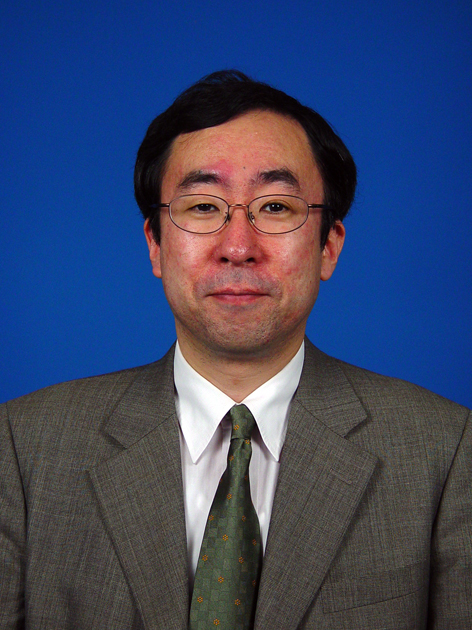
\includegraphics[height=50mm]{data/matsui.jpg}
			\end{figure}
		\end{column}
	\end{columns}\blfootnote{\scriptsize Image: \url{http://www.isce2009.ryukoku.ac.jp/eng/keynote_address.html}}
\end{frame}

\begin{frame}{Linear Approximations}{Introduction}
	\vspace{-10pt}
	\visible<1->{%
	\begin{itemize}
		\item We want to linear approximate a function $F : \mathbb{F}_2^n \rightarrow \mathbb{F}_2^n$
	\end{itemize}
	}

	\vspace{-10pt}
	\begin{columns}[T]
	\visible<2->{%
		\begin{column}{0.48\textwidth}
			\begin{block}{Dot-Product}
				\begin{equation*}
				\vspace{-2pt}
					\langle \alpha, x \rangle = \bigoplus_{i=0}^{n-1} \alpha_i x_i
				\end{equation*}
			\end{block}
		\end{column}
	}
	\visible<3->{%
		\begin{column}{0.48\textwidth}
			\begin{block}{Mask}
				Let $\alpha, \beta, x \in \mathbb{F}_2^n$ and
				%\vspace{-6pt}
				\begin{equation}
					\langle \alpha, x \rangle = \langle \beta, F(x) \rangle \label{equ:masks}
				\end{equation}
			\end{block}
		\end{column}
	}
	\end{columns}

	\visible<3->{%
	\begin{itemize}
		\item We say $\alpha$ is an \emph{input mask} and $\beta$ is an \emph{output mask}.
		\item Equation~\ref{equ:masks} does not hold for every input/output masks.
	\end{itemize}
	}
	\vspace{1em}
	\visible<4->{%
	\begin{itemize}
		\item It is \emph{correlated}, i.e., $\text{Pr}[\langle \alpha, x \rangle = \langle
			\beta, F(x) \rangle] = \frac{c(\alpha, \beta) - 1}{2}$.
	\end{itemize}
	}
\end{frame}

\begin{frame}{LC Example: \spresent/}{Introduction}
	\only<-4>{%
		\begin{columns}[T]
			\begin{column}{0.50\textwidth}
			\only<-2>{%
				\begin{block}{\spresent/-$\bracket*{4}$ over 3 Rounds}
					\centering
					\includegraphics[width=\maxwidth{.75\textwidth},
									height=\maxheight{.75\textheight},
									keepaspectratio]%
									{data/plots/smallpresent4_3r.pdf}
				\end{block}
			}
			\only<3-4>{%
				\begin{block}{\spresent/-$\bracket*{4}$ over 3 Rounds}
					\centering
					\includegraphics[width=\maxwidth{.75\textwidth},
									height=\maxheight{.75\textheight},
									keepaspectratio]%
									{data/plots/smallpresent4_3r_hl.pdf}
				\end{block}
			}
			\end{column}
			\begin{column}{0.48\textwidth}
			\vspace{1cm}
			\visible<2-4>{%
				Basically approximate:
				\begin{itemize}
						\item the \subbox/
						\item the linear layer
				\end{itemize}
			}
			\vspace{1em}
			\visible<4>{%
				\begin{itemize}
						\item the linear layer \enquote{is easy}
						\item for the \subboxes/ use \emph{Linear Approximation Table (LAT)}
				\end{itemize}
			}
			\end{column}
		\end{columns}
	}

	\only<5->{%
		\begin{block}{LAT}
			\robustify\diagbox
			\robustify\hphantom
			\centering
			\scriptsize
			\vspace{1em}
			\tabcolsep=-2pt
			\begin{tabular}{SSSSSSSSSSSSSSSSS}
				\toprule
				\diagbox{$\beta$\hphantom{.}}{\hphantom{.}$\alpha$}&
				    1& 2& 3& 4& 5& 6& 7& 8& 9&10&11&12&13&14&15 \\
				1 &  &  &  &  &-8&  &-8&  &  &  &  &  &-8&  & 8 \\
				2 &  & 4& 4&-4&-4&  &  & 4&-4&  & 8&  & 8&-4&-4 \\
				3 &  & 4& 4& 4&-4&-8&  &-4& 4&-8&  &  &  &-4& 4 \\
				4 &  &-4& 4&-4&-4&  & 8&-4&-4&  &-8&  &  &-4&   \\
				5 &  &-4& 4&-4& 4&  &  & 4& 4&-8&  & 8&  & 4&   \\
				6 &  &  &-8&  &  &-8&  &  &-8&  &  & 8&  &  &-4 \\
				7 &  &  & 8& 8&  &  &  &  &-8&  &  &  &  & 8&-4 \\
				8 &  & 4&-4&  &  &-4& 4&-4& 4&  &  &-4& 4& 8&-4 \\
				9 & 8&-4&-4&  &  & 4&-4&-4&-4&-8&  &-4& 4&  & 4 \\
				10&  & 8&  & 4& 4& 4&-4&  &  &  &-8& 4& 4&-4& 8 \\
				11&-8&  &  &-4&-4& 4&-4&-8&  &  &  & 4& 4& 4&   \\
				12&  &  &  &-4&-4&-4&-4& 8&  &  &-8&-4& 4& 4& 4 \\
				13& 8& 8&  &-4&-4& 4& 4&  &  &  &  & 4&-4& 4& 4 \\
				14&  & 4& 4&-8& 8&-4&-4&-4&-4&  &  &-4&-4&  &   \\
				15& 8& 4&-4& 4& 4&  &  & 8&  & 4&-4&-4&-4&  &   \\
				\bottomrule
			\end{tabular}
			\vspace{1em}
		\end{block}
	}
\end{frame}

\begin{frame}{Linear Hull}{Introduction}
	\visible<1->{%
		\begin{itemize}
			\item Our example exhibits more than one trail for $(\alpha, \beta) = (15, 15)$
			\item Key dependency
		\end{itemize}
	}
	\visible<2->{%
		\begin{block}{Linear Hull}
			Let $F : \mathbb{F}_2^n \rightarrow \mathbb{F}_2^n$ be a block cipher over $r$~rounds,\newline
			and $E : \mathbb{F}_2^m \rightarrow {\left(\mathbb{F}_2^n\right)}^{r+1}$ a key schedule.
			The \emph{linear hull} $c_F^k(\alpha,\beta)$ is
			\begin{equation*}
				c_F^k(\alpha,\beta) := \sum_{\theta|\theta_0=\alpha,\theta_r=\beta} {(-1)}^{\langle \theta, E(k) \rangle} c_\theta
			\end{equation*}
		\end{block}
	}
\end{frame}

\begin{frame}{Distributions}{Introduction}
	\visible<1->{%
	\begin{itemize}
		\item Attack complexity of linear cryptanalysis is proportional to $\left(c_\theta\right)^{-2}$.
	\end{itemize}
	}
	\vspace{1em}
	\visible<2->{%
	\begin{itemize}
		\item We assume the \emph{Hypothesis of Stochastic equivalence}.
		\item Thus, distribution of linear biases follows a normal distribution.
		\item Its width is defined by the variance.
	\end{itemize}
	}
	\vspace{1em}
	\visible<3->{%
	\begin{itemize}
		\item What happens with different key schedules?
	\end{itemize}
	}
\end{frame}

\section{Experiments}
\begin{frame}{\spresent/ variants}{Experiments}
	\begin{columns}
		\begin{column}{0.40\textwidth}
			\begin{block}{Independent Round Keys}
				\centering
				\includegraphics[width=\maxwidth{\textwidth},
								height=\maxheight{.55\textheight},
								keepaspectratio]%
								{data/plots/independent_round_keys.pdf}
			\end{block}
		\end{column}
		\begin{column}{0.40\textwidth}
			\begin{block}{Constant Round Keys}
				\centering
				\includegraphics[width=\maxwidth{\textwidth},
								height=\maxheight{.55\textheight},
								keepaspectratio]%
								{data/plots/constant_round_keys.pdf}
			\end{block}
		\end{column}
	\end{columns}
	\begin{columns}
		\begin{column}{0.50\textwidth}
			\begin{block}{\subboxes/}
				\centering
				choose $S \in \curly*{R_0, \ldots, R_{19}}$
			\end{block}
		\end{column}
	\end{columns}
\end{frame}

\section{Results}
\begin{frame}{Distributions}{Results}
	\only<1>{%
		\begin{block}{\spresent/-$\bracket*{16}$ with $R_0$, 10 rounds}
			\centering
			\vspace{1em}
			\includegraphics[width=\maxwidth{\textwidth},
			height=\maxheight{.55\textheight},
			keepaspectratio]%
			{data/plots/sbox_serpent0_16n_10r.pdf}
			\vspace{1em}
		\end{block}
	}

	\only<2>{%
		\begin{block}{\spresent/-$\bracket*{16}$ with $R_1$, 10 rounds}
			\centering
			\vspace{1em}
			\includegraphics[width=\maxwidth{\textwidth},
			height=\maxheight{.55\textheight},
			keepaspectratio]%
			{data/plots/sbox_serpent1_16n_10r.pdf}
			\vspace{1em}
		\end{block}
	}

	\only<3>{%
		\begin{block}{\spresent/-$\bracket*{16}$ with $R_2$, 10 rounds}
			\centering
			\vspace{1em}
			\includegraphics[width=\maxwidth{\textwidth},
			height=\maxheight{.55\textheight},
			keepaspectratio]%
			{data/plots/sbox_serpent2_16n_10r.pdf}
			\vspace{1em}
		\end{block}
	}

	\only<4>{%
		\begin{block}{\spresent/-$\bracket*{16}$ with $R_2$, 11 rounds}
			\centering
			\vspace{1em}
			\includegraphics[width=\maxwidth{\textwidth},
			height=\maxheight{.55\textheight},
			keepaspectratio]%
			{data/plots/sbox_serpent2_16n_11r.pdf}
			\vspace{1em}
		\end{block}
	}
\end{frame}

\begin{frame}{More Distributions for $R_1$}{Results}
	\foreach \plotindex in {10,...,25}{%
		\pgfmathparse{\plotindex-9}
		\pgfmathroundto{\pgfmathresult}
		\only<\pgfmathresult>{%
			\begin{block}{\spresent/-$\bracket*{16}$ with $R_1$, \plotindex\ rounds}
				\centering
				\vspace{1em}
				\includegraphics[width=\maxwidth{\textwidth},
				height=\maxheight{.55\textheight},
				keepaspectratio]%
				{data/plots/sbox_R1_0\plotindex_256keys.pdf}
				\vspace{1em}
			\end{block}
		}
	}
\end{frame}

\begin{frame}{Behaviour over more rounds}{Results}
	\begin{block}{Min/Max correlation with \subbox/ $R_1$, normalised to standard deviations}
		\centering
		\vspace{1em}
		\includegraphics[width=\maxwidth{\textwidth},
		height=\maxheight{.55\textheight},
		keepaspectratio]%
		{data/plots/convergence_r1.pdf}
		\vspace{1em}
	\end{block}
\end{frame}

\begin{frame}{Induced Graph}{Results}
	\only<-1>{%
	\begin{columns}
		\begin{column}{0.48\textwidth}
			\begin{block}{\spresent/-$\bracket*{4}$}
				\centering
				\vspace{1em}
				\includegraphics[width=\maxwidth{\textwidth},
				height=\maxheight{.55\textheight},
				keepaspectratio]%
				{data/plots/smallpresent4.pdf}
				\vspace{1em}
			\end{block}
		\end{column}
		\begin{column}{0.5\textwidth}
			\begin{itemize}
				\item adjacency matrix from ciphers round function
				\item each bit is a vertex
				\item each non-zero entry in the LAT is an edge
			\end{itemize}
		\end{column}
	\end{columns}
	}
	\only<2->{%
	\begin{columns}
		\begin{column}{0.3\textwidth}
			\begin{block}{\subbox/ $R_0$}
				\centering
				\vspace{1em}
				\includegraphics[width=\maxwidth{\textwidth},
				height=\maxheight{.65\textheight},
				keepaspectratio]%
				{data/plots/sbox_serpent0_16n_10r_graph_inkscape.pdf}
				\vspace{1em}
			\end{block}
		\end{column}
		\begin{column}{0.3\textwidth}
			\begin{block}{\subbox/ $R_1$}
				\centering
				\vspace{1em}
				\includegraphics[width=\maxwidth{\textwidth},
				height=\maxheight{.65\textheight},
				keepaspectratio]%
				{data/plots/sbox_serpent1_16n_10r_graph_inkscape.pdf}
				\vspace{1em}
			\end{block}
		\end{column}
		\begin{column}{0.3\textwidth}
			\begin{block}{\subbox/ $R_2$}
				\centering
				\vspace{1em}
				\includegraphics[width=\maxwidth{\textwidth},
				height=\maxheight{.65\textheight},
				keepaspectratio]%
				{data/plots/sbox_serpent2_16n_10r_graph_inkscape.pdf}
				\vspace{1em}
			\end{block}
		\end{column}
	\end{columns}
	}
\end{frame}


\section{Future Work}
\begin{frame}{A new (un-) secure \present/ variant}{Future Work}
	\visible<1->{%
		\begin{block}{Proposal}
			\begin{itemize}
				\item \present/ with $R_2$ as \subbox/
				\item 31 encryption rounds
				\item Constant key schedule
			\end{itemize}
		\end{block}
	}

	\visible<2->{%
		\begin{alertblock}{Problem: Constant key schedule is suspicious}
			\begin{itemize}
				\item Slide attacks
				\item Wider distribution is known
			\end{itemize}
		\end{alertblock}
	}
\end{frame}

\begin{frame}{Future Work}
	\visible<1->{%
		\begin{block}{Invariant Subspaces (Inv.\,Subs) in Key Schedules}
			\begin{itemize}
				\item Invariant subspaces can be equivalent to constant round keys.
				\item Can we construct functions with specific Inv.\,Subs?
				\item Is there an unsuspicious key schedule with an Inv.\,Sub?
			\end{itemize}
		\end{block}
	}

	\visible<2->{%
		\begin{block}{Hypothesis of Stochastic Equivalence}
			\begin{itemize}
				\item Find an explanation for observed behaviour.
			\end{itemize}
		\end{block}
	}

	\visible<3->{%
		\begin{block}{Hypothesis of Wrong Key Randomisation}
			\begin{itemize}
				\item Scrutinise wrong key behaviour.
			\end{itemize}
		\end{block}
	}
\end{frame}


\begin{frame}{Questions?}{Thank you for your attention!}
	\begin{figure}[!htb]
		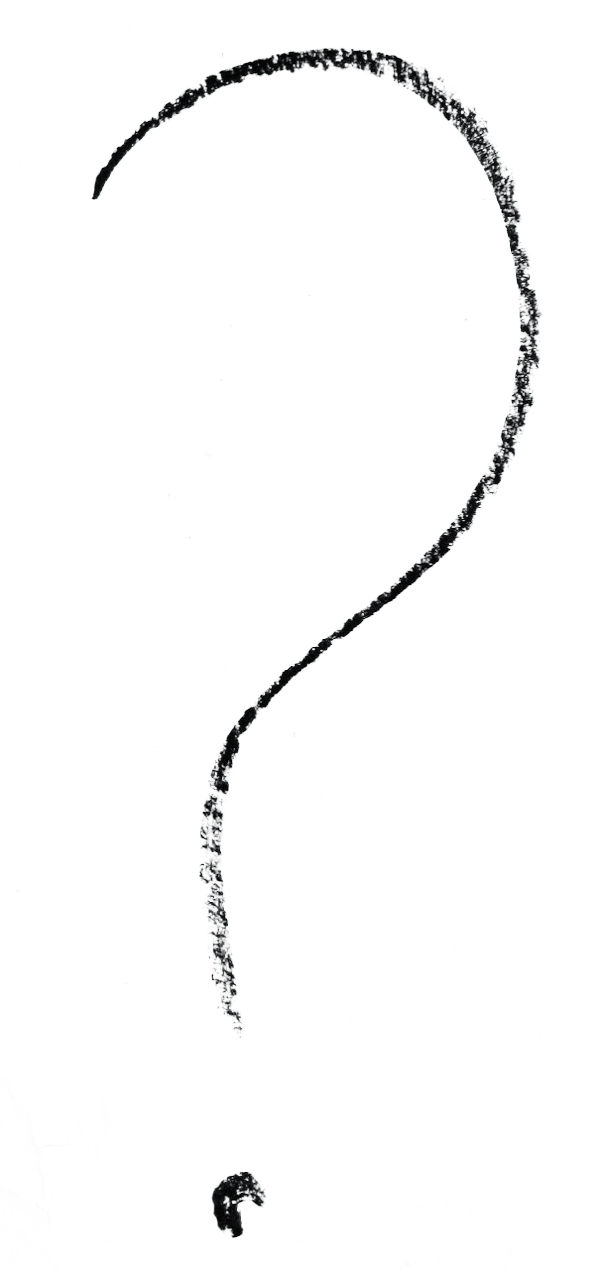
\includegraphics[height=50mm]{data/flickr/questionmark.png}\blfootnote{\scriptsize Mainboard \& Questionmark Images: flickr}
	\end{figure}
\end{frame}

%\begin{frame}{References}
%	\tiny
%	\printbibliography{}
%\end{frame}

\end{document}
